% Provenance (never printed): see sources/outline_sources.md (Year 2: viscosity, density and
% volatiles of magmas; magma ascent; dykes, sills and plutons; contact aureoles).
% Curves from figdata/bachelor-2/magma.py (GRD 2008 viscosity, DensityX density, Moore 1998
% solubility data, erf sill cooling, Stefan solidification); exercise and problem values in
% the Book 4 scratch calculators calc/ch05.py and calc/ch05pb.py.
\chapter{Magma's en hun intrusie}\label{ch:b2:magma-emplacement}

Een basaltsmelt van \qty{1200}{\celsius} vloeit met een viscositeit van ongeveer
\qty{70}{Pa.s}: stroperig, maar hij laat zich gieten. Een droge rhyolietsmelt van \qty{800}{\celsius}
heeft een viscositeit van bijna \qty{e11}{Pa.s}, en een blok ervan zou uren nodig hebben om
zichtbaar onder zijn eigen gewicht door te zakken. Daartussen liggen tien grootteordes, meer
dan tussen water en het basalt, en het grootste deel van het verschil komt van twee
dingen: het silica dat de smelt tot een netwerk verbindt, en de temperatuur,
die in silicarijke \omterm{def:b2:magma-emplacement:magma}{magma's} enkele honderden graden lager is. Enkele procenten
opgelost water, die een rhyolietmagma op diepte kan bevatten, verlagen zijn viscositeit
met een factor \num{e5}, en die winst gaat weer verloren als het \omterm{def:b2:magma-emplacement:magma}{magma} opstijgt en het
water als bellen vrijkomt. Deze getallen bepalen of een \omterm{def:b2:magma-emplacement:magma}{magma} rustig het
oppervlak bereikt, explodeert, of kilometers diep stolt als een \omterm{def:b2:magma-emplacement:bodies}{gang}, een \omterm{def:b2:magma-emplacement:bodies}{sill} of een
\omterm{def:b2:magma-emplacement:bodies}{pluton}. Dit hoofdstuk behandelt een \omterm{def:b2:magma-emplacement:magma}{magma} als een materiaal: zijn dichtheid, viscositeit en
vluchtige bestanddelen, de fysica van zijn opstijging door spleten en als bellen, de vormen die het
aanneemt wanneer het stopt, en de warmte die het aan de omringende gesteenten afgeeft.
% ledger: grd08:model, grd08:range, moore98:melts

\begin{recall}
\textbf{Viskeuze stroming} (natuurkunde, tweede jaar universiteit): in een newtonse vloeistof met
viscositeit $\eta$ is de schuifspanning $\eta$ maal de snelheidsgradiënt; tussen
twee evenwijdige wanden drijft een drukgradiënt een parabolisch profiel (vlakke Poiseuille-stroming)
aan; een bol die langzaam door een viskeuze vloeistof beweegt, ondervindt de stokeswrijving
$6\pi\eta a v$. \textbf{Warmtegeleiding} (zelfde jaar): de temperatuur voldoet aan
$\partial T/\partial t = \kappa\,\partial^2T/\partial x^2$, met diffusiviteit $\kappa = k/(\rho
c)$, en een temperatuursprong spreidt zich als een foutfunctie uit over een afstand van
de orde $\sqrt{\kappa t}$. \textbf{Opwaartse kracht} (natuurkunde, eerste jaar universiteit): een lichaam
dat in een dichtere vloeistof is ondergedompeld, ondervindt een netto opwaartse kracht gelijk aan het gewicht van de
verplaatste vloeistof min zijn eigen gewicht. \textbf{Chemisch evenwicht} (scheikunde): in
evenwicht voldoen de activiteiten van producten en reactanten aan de massawerkingswet
met een constante $K$ die van de temperatuur afhangt. Uit Boek~3
van deze reeks: de lithostatische druk $p = \rho g z$ en de geotherm; uit de
Boeken 1 en 2: mafische en felsische gesteenten, fenokristen en porfirische texturen.
\end{recall}

\section{Wat een magma is}

\begin{definition}[Magma]\label{def:b2:magma-emplacement:magma}
Een \emph{magma}\index{magma} is gesmolten of gedeeltelijk gesmolten gesteente onder het oppervlak: een
\emph{silicaatsmelt}\index{silicaatsmelt}, de vloeistof die vooral uit silicium,
zuurstof en metaalkationen bestaat, samen met de kristallen en gasbellen die ze meevoert.
Een \emph{kristalbrij}\index{kristalbrij} is een magma dat zo rijk is aan kristallen dat ze
elkaar raken en een raamwerk vormen: het kan niet als een vloeistof stromen, en zijn smelt kan alleen
door de poriën tussen de kristallen bewegen.
\end{definition}

De samenstelling van de smelt wordt, zoals voor gesteenten, gegeven in gewichtsprocent
oxiden. Drie smelten dienen het hele hoofdstuk door als referentie, alle drie
in het laboratorium bestudeerd: een tholeïtisch basalt dat van een mid-oceanische rug is opgedregd
(ongeveer \qty{51}{\percent} SiO$_2$, \qty{12}{\percent} ijzeroxide, \qty{7}{\percent}
MgO), een andesiet (\qty{63}{\percent} SiO$_2$) en een rhyoliet (\qty{78}{\percent}
SiO$_2$, \qty{8}{\percent} Na$_2$O $+$ K$_2$O en bijna geen ijzer of magnesium).
Hun eruptietemperaturen verschillen evenveel als hun samenstellingen: basaltische
\omterm{def:b2:magma-emplacement:magma}{magma's} komen tot uitbarsting bij \qtyrange{1000}{1200}{\celsius} (lava die door een lavatunnel op
Kilauea stroomde, is bij bijna \qty{1200}{\celsius} gemeten), andesitische \omterm{def:b2:magma-emplacement:magma}{magma's} bij
\qtyrange{800}{1000}{\celsius}, rhyolitische \omterm{def:b2:magma-emplacement:magma}{magma's} bij \qtyrange{650}{800}{\celsius}.
Een rhyolitisch \omterm{def:b2:magma-emplacement:magma}{magma} is koeler omdat het het residu is van een lange kristallisatie
of de eerste smelt van korstgesteenten, die allebei bij lage temperatuur plaatsvinden
(\cref{ch:b2:magmatic-differentiation}).
% ledger: moore98:melts, tulane:magma-types, earle:kilauea-lava

Het kristalgehalte bepaalt of een \omterm{def:b2:magma-emplacement:magma}{magma} stroomt. Veld- en geochronologische
studies van grote granietlichamen concluderen dat magmatische stroming in bulk een
smeltfractie van minstens \qtyrange{30}{50}{\percent} in volume vraagt; daaronder zijn de
kristallen aan hun buren vastgegroeid en vervormt het materiaal als een vaste stof met
poriën vol smelt. Een groot deel van het \omterm{def:b2:magma-emplacement:magma}{magma} dat in de korst is opgeslagen, verkeert vermoedelijk in
die toestand, als een brij die weer mobiel wordt wanneer er van onderen heet \omterm{def:b2:magma-emplacement:magma}{magma}
bijkomt.
% ledger: glazner04:tuolumne

\section{Dichtheid en viscositeit}

\subsection{De dichtheid van een smelt}

Een \omterm{def:b2:magma-emplacement:magma}{silicaatsmelt} heeft geen kristalrooster, maar zijn volume kan toch worden opgebouwd uit
zijn componenten. Experimenten met veel smelten tonen dat elk oxide een
bijna vast volume per mol bijdraagt, zijn partieel molair volume, dat langzaam en
lineair met temperatuur en druk verandert; het volume van de smelt is de som van
deze bijdragen. De tabel hieronder geeft de waarden die in dit hoofdstuk worden gebruikt.

\begin{table}[ht]
\centering\small
\begin{tabular}{lrrr}
\hline
Oxide & $\bar V_i$ (\unit{cm^3/mol}) & $\partial\bar V_i/\partial T$ (\num{e-3}\,\unit{cm^3/(mol.K)}) & $\partial\bar V_i/\partial p$ (\num{e-4}\,\unit{cm^3/(mol.bar)}) \\
\hline
SiO$_2$  & 26.86 & 0     & $-1.89$ \\
Al$_2$O$_3$ & 37.42 & 2.62 & $-2.26$ \\
FeO      & 12.68 & 3.69  & $-0.45$ \\
MgO      & 12.02 & 3.27  & $0.27$ \\
CaO      & 16.90 & 3.74  & $0.34$ \\
Na$_2$O  & 29.65 & 7.68  & $-2.40$ \\
K$_2$O   & 47.28 & 12.08 & $-6.75$ \\
H$_2$O   & 22.9  & 9.5   & $-3.20$ \\
\hline
\end{tabular}
\caption{Partiële molaire volumes van oxidecomponenten in \omterm{def:b2:magma-emplacement:magma}{silicaatsmelten} bij
\qty{1}{bar}, met hun afgeleiden naar temperatuur en druk. De
referentietemperatuur is \qty{1773}{K} (FeO \qty{1723}{K}, H$_2$O \qty{1273}{K}). Gegevens:
compilatie van het programma DensityX (Iacovino en Till, 2019).}
\label{tab:b2:magma-emplacement:volumes}
\end{table}
% ledger: densityx:volumes

\begin{proposition}[Dichtheid van een silicaatsmelt]\label{prop:b2:magma-emplacement:density}
Laat een smelt oxidecomponenten $i$ bevatten met molfracties $X_i$, molaire massa's
$M_i$ en partiële molaire volumes $\bar V_i(T, p) = \bar V_i^{\circ} + (\partial\bar
V_i/\partial T)(T - T_{\mathrm{ref}}) + (\partial\bar V_i/\partial p)(p - p_{\mathrm{ref}})$.
Als de componenten ideaal mengen in volume, geldt
\[
\rho = \frac{\sum_i X_i M_i}{\sum_i X_i \bar V_i(T,p)}.
\]
\end{proposition}

\begin{proof}
Eén mol smelt bevat $X_i$ mol van component $i$, met massa $X_iM_i$. Ideale
menging in volume betekent dat elke mol van component $i$ het volume $\bar V_i$ toevoegt,
wat de andere ook zijn, dus de mol smelt neemt $\sum_i X_i\bar V_i$ in. De
dichtheid is de verhouding van de twee.
\end{proof}

Water heeft een molaire massa van slechts \qty{18}{g/mol} maar een partieel molair volume van
\qty{22.9}{cm^3/mol}, dicht bij dat van silica: het verlaagt de dichtheid van een smelt
sterk. Toegepast op de drie referentiesmelten geeft de propositie
\qty{2730}{kg/m^3} voor het basalt bij \qty{1200}{\celsius}, \qty{2480}{kg/m^3} voor
het andesiet bij \qty{1000}{\celsius} en \qty{2340}{kg/m^3} voor het droge rhyoliet
bij \qty{850}{\celsius}; één procent opgelost water haalt ongeveer
\qty{70}{kg/m^3} van het basalt af, evenveel als enkele honderden graden verwarming.
Een basaltsmelt is daarom lichter dan het mantelperidotiet waaruit hij komt
(ongeveer \qty{3380}{kg/m^3} onder de korst in het referentiemodel van de aarde) en een
beetje lichter dan de onderkorst van dat model (\qty{2900}{kg/m^3}), terwijl een
rhyolietsmelt zelfs lichter is dan de bovenkorst ervan (\qty{2600}{kg/m^3}). Dit verschil drijft \omterm{def:b2:magma-emplacement:magma}{magma's}
omhoog.
% ledger: densityx:volumes, densityx:water, data:prem

\subsection{Viscositeit}

De viscositeit van een \omterm{def:b2:magma-emplacement:magma}{silicaatsmelt} wordt bepaald door het netwerk van SiO$_4$-tetraëders
die via gedeelde zuurstofatomen verbonden zijn: om te stromen moet de smelt
silicium--zuurstofbindingen verbreken en opnieuw vormen. Silica en alumina bouwen het netwerk; de kationen van
magnesium, ijzer, calcium en de alkalimetalen breken het, en water ook, dat
brugvormende zuurstofatomen in hydroxylgroepen omzet. Laboratoriummetingen aan natuurlijke
smelten beslaan meer dan vijftien grootteordes, van \qty{0.1}{Pa.s} tot
\qty{e14}{Pa.s}, en ze volgen geen eenvoudige arrheniuswet: de viscositeit
stijgt sneller dan exponentieel in $1/T$ naarmate de smelt afkoelt naar zijn
glasovergang.
% ledger: grd08:range

\begin{proposition}[Wet van Vogel--Fulcher--Tammann]\label{prop:b2:magma-emplacement:vft}
De viscositeit van een \omterm{def:b2:magma-emplacement:magma}{silicaatsmelt} met vaste samenstelling volgt, binnen enkele
tienden van een logaritmische eenheid,
\[
\log_{10}\eta = A + \frac{B}{T - C},
\]
met $\eta$ in pascalseconde en $T$ in kelvin. Voor natuurlijke smelten ligt $A$ dicht
bij $-4.55$, wat de samenstelling ook is; $B$ en $C$ (in kelvin) zijn lineaire
combinaties van de molpercentages van de oxiden, met enkele producten ervan,
gefit op ongeveer \num{1800} metingen.
\end{proposition}
\admitted
% ledger: grd08:model, grd08:range

De figuur hieronder toont de wet voor de drie referentiesmelten en voor het
rhyoliet met opgelost water. Bij \qty{1200}{\celsius} heeft het basalt
$\eta \approx \qty{70}{Pa.s}$; het andesiet bij \qty{1000}{\celsius} ongeveer
\qty{e6}{Pa.s}; het droge rhyoliet bij \qty{800}{\celsius} ongeveer $10^{10.9}$\,\unit{Pa.s}.
Vier procent water brengt hetzelfde rhyoliet terug tot $10^{5.5}$\,\unit{Pa.s}, zes
procent tot $10^{4.6}$\,\unit{Pa.s}. Een onafhankelijke vergelijking, alleen gefit op waterhoudende
granitische smelten, geeft dezelfde waarden binnen een halve logaritmische eenheid
(\cref{exo:b2:magma-emplacement:1}). Het effect van water is het grootst bij lage temperatuur, waar enkele
tienden van een procent de viscositeit met grootteordes veranderen.
% ledger: grd08:model, hd96:model, moore98:melts

\begin{omfigure}
\centering
\begin{tikzpicture}
\begin{axis}[omrecord, width=0.86\linewidth, height=6.4cm,
  xmin=600, xmax=1400, ymin=0, ymax=15,
  xlabel={temperatuur (\unit{\celsius})}, ylabel={$\log_{10}\eta$ (\unit{Pa.s})},
  legend pos=north east, legend style={font=\scriptsize},
  tick label style={font=\scriptsize}, label style={font=\small}]
\addplot[very thick, black, restrict x to domain=1000:1400] table[x=T_C, y=basalt] {figdata/out/bachelor-2-magma-visc.dat};
\addlegendentry{basalt, droog}
\addplot[very thick, brown, restrict x to domain=800:1300] table[x=T_C, y=andesite] {figdata/out/bachelor-2-magma-visc.dat};
\addlegendentry{andesiet, droog}
\addplot[very thick, red!70!black, restrict x to domain=650:1100] table[x=T_C, y=rhyolite] {figdata/out/bachelor-2-magma-visc.dat};
\addlegendentry{rhyoliet, droog}
\addplot[thick, red!70!black, dashed, restrict x to domain=650:1000] table[x=T_C, y=rhy2] {figdata/out/bachelor-2-magma-visc.dat};
\addlegendentry{rhyoliet, 2 \% H$_2$O}
\addplot[thick, red!70!black, densely dotted, restrict x to domain=650:1000] table[x=T_C, y=rhy4] {figdata/out/bachelor-2-magma-visc.dat};
\addlegendentry{rhyoliet, 4 \% H$_2$O}
\addplot[thick, red!70!black, dashdotted, restrict x to domain=650:1000] table[x=T_C, y=rhy6] {figdata/out/bachelor-2-magma-visc.dat};
\addlegendentry{rhyoliet, 6 \% H$_2$O}
\end{axis}
\end{tikzpicture}
\par\smallskip{\small Viscositeit van \omterm{def:b2:magma-emplacement:magma}{silicaatsmelten} tegen de temperatuur, volgens de
wet van Vogel--Fulcher--Tammann met de van de samenstelling afhankelijke parameters van
Giordano, Russell en Dingwell (2008). Basalt: een tholeïet van een mid-oceanische rug;
andesiet en rhyoliet: referentiesmelten uit het laboratorium (Moore en anderen, 1998). Elke
kromme is getekend over de temperaturen waarbij zo'n \omterm{def:b2:magma-emplacement:magma}{magma} gesmolten kan zijn.}
\end{omfigure}
% ledger: grd08:model, moore98:melts

Kristallen maken een \omterm{def:b2:magma-emplacement:magma}{magma} nog stijver. Een suspensie van starre deeltjes verzet zich
sterker tegen afschuiving dan haar vloeistof alleen, omdat de vloeistof om de
deeltjes heen moet stromen, en wanneer de deeltjes dicht genoeg opeengepakt zijn om elkaar te raken, vergrendelen ze tot een
raamwerk.

\begin{proposition}[Relatie van Einstein--Roscoe]\label{prop:b2:magma-emplacement:roscoe}
Een suspensie van een volumefractie $\phi$ starre bollen in een newtonse vloeistof
met viscositeit $\eta_{\ell}$ heeft de viscositeit
\[
\eta = \eta_{\ell}\,(1 - R\phi)^{-2.5}, \qquad R = 1/\phi_m \approx 1.35,
\]
waarbij $\phi_m$ de maximale pakkingsfractie is, waarbij de suspensie vastloopt. Voor
kleine $\phi$ wordt dit de relatie van Einstein, $\eta = \eta_{\ell}(1 + 2.5\phi)$.
\end{proposition}
\admitted
% ledger: kolz22:einstein-roscoe

Twintig procent kristallen verdubbelt de viscositeit, veertig procent vermenigvuldigt haar met
zeven, zestig procent met meer dan zestig (\cref{exo:b2:magma-emplacement:5}); in echte \omterm{def:b2:magma-emplacement:magma}{magma's}, waar de
kristallen langwerpig en van veel groottes zijn, komt de vergrendeling eerder, rond de
\qtyrange{50}{70}{\percent} kristallen waarbij de veldgegevens het
einde van de stroming in bulk plaatsen.

\section{Vluchtige bestanddelen}

\begin{definition}[Magmatische vluchtige bestanddelen]\label{def:b2:magma-emplacement:volatiles}
Een \emph{magmatisch vluchtig bestanddeel}\index{magmatisch vluchtig bestanddeel} is een component van een \omterm{def:b2:magma-emplacement:magma}{magma} dat
op diepte in de smelt is opgelost en bij lage druk een aparte gasfase vormt:
vooral water, dan koolstofdioxide, dan zwavelverbindingen. \emph{Ontmenging van vluchtige
bestanddelen}\index{ontmenging van vluchtige bestanddelen} is de scheiding van een vluchtig bestanddeel uit de
smelt in gasbellen. De \emph{verzadigingsdruk van vluchtige
bestanddelen}\index{verzadigingsdruk van vluchtige bestanddelen} van een smelt is de druk waaronder
zijn opgeloste vluchtige bestanddelen hun oplosbaarheid overschrijden, zodat zich een gasfase moet vormen.
\end{definition}

Mafische \omterm{def:b2:magma-emplacement:magma}{magma's} bevatten gewoonlijk \qtyrange{1}{3}{\percent} vluchtige bestanddelen in massa,
intermediaire \omterm{def:b2:magma-emplacement:magma}{magma's} \qtyrange{3}{4}{\percent}, felsische \omterm{def:b2:magma-emplacement:magma}{magma's}
\qtyrange{4}{7}{\percent}, en de ontmenging van \qtyrange{4}{6}{\percent}
water drijft de meeste explosieve erupties aan. Hoeveel water een smelt kan bevatten, hangt
vooral van de druk af. De figuur hieronder toont metingen aan basaltische en
rhyolitische smelten die bij een bekende waterdruk werden gehouden tot ze verzadigd waren, daarna tot glas
afgeschrikt en geanalyseerd: de oplosbaarheid stijgt steil bij lage druk en
trager bij hoge druk.
% ledger: earle:volatiles, moore98:arc-water, moore98:h2o

\begin{proposition}[Wortelwet voor water]\label{prop:b2:magma-emplacement:sqrt}
Veronderstel dat water in een \omterm{def:b2:magma-emplacement:magma}{silicaatsmelt} vooral als hydroxylgroepen oplost, via
de reactie $\mathrm{H_2O\,(gas)} + \mathrm{O^{2-}\,(melt)} \rightleftharpoons
2\,\mathrm{OH^-\,(melt)}$, met de zuurstof van de smelt in grote overmaat. Dan is,
bij lage watergehalten, het opgeloste water evenredig met de vierkantswortel van
de waterdruk: $w \approx s\sqrt{p}$, met $s$ een constante die afhangt van de smelt en de
temperatuur.
\end{proposition}

\begin{proof}
De massawerkingswet geeft $x_{\mathrm{OH}}^2 = K\,x_{\mathrm{O}}\,f$, waarbij $f$
de fugaciteit van water is (bij matige drukken dicht bij zijn druk) en de $x$
molfracties zijn. De zuurstof van de smelt is in grote overmaat, dus
$x_{\mathrm{O}}$ blijft bijna constant, en $x_{\mathrm{OH}} = \sqrt{Kx_{\mathrm{O}}}\,
\sqrt f$. Elke opgeloste watermolecule vormt twee hydroxylgroepen, dus het opgeloste
water is $x_{\mathrm{OH}}/2$, evenredig met $\sqrt f$. Bij hogere gehalten lost een deel
van het water op als moleculen, evenredig met $f$ zelf, en stijgt de
oplosbaarheid sneller dan de vierkantswortel (\cref{exo:b2:magma-emplacement:10}).
\end{proof}

Met de kleinste kwadraten op de metingen gefit, geeft $w = s\sqrt p$
$s = 0.34$ gewichtsprocent per $\sqrt{\unit{MPa}}$ voor de basalten en
$s = 0.44$ voor de rhyolieten; elke meting ligt binnen één procent
water van haar kromme. De verzadigingsdruk van een smelt met $w$ procent
water is dan $p_s = (w/s)^2$: \qty{129}{MPa} voor een rhyoliet met
\qty{5}{\percent} water, ongeveer \qty{5}{km} diep in de korst, maar slechts
\qty{2}{MPa} voor een basalt met \qty{0.5}{\percent}, honderd meter of minder.
% ledger: moore98:h2o

\begin{omfigure}
\centering
\begin{tikzpicture}
\begin{axis}[omrecord, width=0.8\linewidth, height=6cm,
  xmin=0, xmax=300, ymin=0, ymax=9,
  xlabel={waterdruk (\unit{MPa})}, ylabel={opgelost H$_2$O (gew.-\%)},
  legend pos=south east, legend style={font=\scriptsize},
  tick label style={font=\scriptsize}, label style={font=\small}]
\addplot[very thick, red!70!black] table[x=P_MPa, y=rhyolite] {figdata/out/bachelor-2-magma-solub-fit.dat};
\addlegendentry{rhyoliet, $0.44\sqrt p$}
\addplot[only marks, mark=*, mark size=2pt, red!70!black] table[x=P_MPa, y=w] {figdata/out/bachelor-2-magma-solub-rhyolite-data.dat};
\addlegendentry{rhyoliet, gemeten}
\addplot[very thick, black] table[x=P_MPa, y=basalt] {figdata/out/bachelor-2-magma-solub-fit.dat};
\addlegendentry{basalt, $0.34\sqrt p$}
\addplot[only marks, mark=square*, mark size=2pt, black] table[x=P_MPa, y=w] {figdata/out/bachelor-2-magma-solub-basalt-data.dat};
\addlegendentry{basalt, gemeten}
\end{axis}
\end{tikzpicture}
\par\smallskip{\small Oplosbaarheid van water in basaltische en rhyolitische smelten bij
\qtyrange{800}{1200}{\celsius} tegen de waterdruk: metingen verzameld
door Moore en anderen (1998), en wortelwetten gefit met de kleinste kwadraten. Bij
\qty{100}{MPa}, ongeveer \qty{4}{km} diep in de korst, kan een rhyoliet
\qty{4.4}{\percent} water bevatten, een basalt \qty{3.4}{\percent}.}
\end{omfigure}
% ledger: moore98:h2o

Koolstofdioxide is veel minder oplosbaar dan water. Het lost op als moleculen in
rhyolieten en als carbonaatgroepen in basalten, meer in alkalische smelten dan in
tholeïeten, en ook zijn oplosbaarheid stijgt met de druk. Een \omterm{def:b2:magma-emplacement:magma}{magma} met beide
gassen begint daarom al diep te ontmengen, met een gas dat zeer rijk is aan CO$_2$, en het
gas wordt rijker aan water naarmate het \omterm{def:b2:magma-emplacement:magma}{magma} opstijgt. Basalten die op de diepe
zeebodem zijn uitgevloeid, bevatten blaasjes met meer dan \qty{95}{\percent} CO$_2$, wat
verzadiging met CO$_2$ vereiste, zelfs onder \qty{5}{km} water. Schattingen van het oorspronkelijke
CO$_2$-gehalte van de moederbasalten van Kilauea lopen van \qtyrange{0.2}{0.6}{\percent},
en smeltinsluitsels die in hun olivijnkristallen zijn opgesloten, leggen
verzadigingsdrukken tot \qty{500}{MPa} vast.
% ledger: lowenstern01:co2, lowenstern01:basalts

Ontmengd gas neemt een groot volume in. Eén procent water in een \omterm{def:b2:magma-emplacement:magma}{magma} van
\qty{900}{\celsius} neemt, als ideaal gas, ongeveer \qty{12}{\percent} van het
volume in bij \qty{100}{MPa}, \qty{57}{\percent} bij \qty{10}{MPa} en meer dan
\qty{99}{\percent} bij atmosferische druk (\cref{exo:b2:magma-emplacement:7}). De bellen verlagen de
dichtheid van het \omterm{def:b2:magma-emplacement:magma}{magma} nog meer en drijven het sneller omhoog; in een viskeus \omterm{def:b2:magma-emplacement:magma}{magma}
kunnen ze niet ontsnappen, en \cref{ch:b2:eruptive-styles} laat zien hoe ze het fragmenteren.

\section{Opstijging}

Een magmalichaam dat minder dicht is dan zijn omgeving, ondervindt een opwaartse kracht van
$\Delta\rho\,g$ per volume-eenheid, waarbij $\Delta\rho$ het dichtheidsverschil is. Het
kan op twee manieren opstijgen: door een spleet die het voor zich uit opent, of als een hete,
zachte bel die het omringende gesteente opzij duwt.

\subsection{Gangen}

Op diepte staat het gesteente onder een grote lithostatische druk, maar een spleet gevuld
met \omterm{def:b2:magma-emplacement:magma}{magma} onder een iets hogere druk dan de kleinste hoofdspanning kan
opengaan en aan haar top langer worden. \omterm{def:b2:magma-emplacement:magma}{Magma} vult de spleet terwijl die groeit, en het resultaat
is een dunne plaat \omterm{def:b2:magma-emplacement:magma}{magma}, meters breed en kilometers lang, die zich een weg
omhoog snijdt: een \omterm{def:b2:magma-emplacement:bodies}{gang} in wording. Het \omterm{def:b2:magma-emplacement:magma}{magma} stroomt dan tussen twee bijna evenwijdige
wanden.

\begin{proposition}[Stroming van magma in een gang]\label{prop:b2:magma-emplacement:poiseuille}
Een newtons \omterm{def:b2:magma-emplacement:magma}{magma} met viscositeit $\eta$ dat door een drukgradiënt $G$ omhoog wordt gedreven
(voor stroming door opwaartse kracht $G = \Delta\rho\,g$) tussen twee evenwijdige wanden op een afstand $w$
van elkaar, stroomt met de gemiddelde snelheid
\[
\bar u = \frac{G w^2}{12\,\eta},
\]
en het volumedebiet per lengte-eenheid van de \omterm{def:b2:magma-emplacement:bodies}{gang} is $q = \bar u w = G w^3/(12\eta)$.
\end{proposition}

\begin{proof}
Bij stationaire laminaire stroming is het snelheidsprofiel over de \omterm{def:b2:magma-emplacement:bodies}{gang} de vlakke
poiseuilleparabool $u(x) = \frac{G}{2\eta}\left(\frac{w^2}{4} - x^2\right)$, voor
$-w/2 \le x \le w/2$, die op beide wanden nul is. Haar gemiddelde is
$\bar u = \frac1w\int_{-w/2}^{w/2}u\,dx = \frac{G}{2\eta}\left(\frac{w^2}{4} -
\frac{w^2}{12}\right) = \frac{Gw^2}{12\eta}$.
\end{proof}

De derde macht van de breedte maakt brede \omterm{def:b2:magma-emplacement:bodies}{gangen} veel efficiënter dan smalle. Een
basalt van \qty{100}{Pa.s} in een \omterm{def:b2:magma-emplacement:bodies}{gang} van \qty{1}{m} breed, met $\Delta\rho =
\qty{300}{kg/m^3}$, stijgt met ongeveer \qty{2.5}{m/s} en doorkruist \qty{10}{km}
korst in een uur; een rhyoliet van \qty{e6}{Pa.s} in dezelfde \omterm{def:b2:magma-emplacement:bodies}{gang} zou er meer
dan een jaar over doen, en onderweg stollen, dus silicarijke \omterm{def:b2:magma-emplacement:magma}{magma's} hebben veel bredere
\omterm{def:b2:magma-emplacement:bodies}{gangen} nodig (\cref{exo:b2:magma-emplacement:6}). Het reynoldsgetal $\rho\bar u w/\eta$ van deze stromingen
is klein genoeg om ze laminair te houden. Opstijgsnelheden die voor \omterm{def:b2:magma-emplacement:magma}{magma's}
tijdens erupties zijn geschat, scheiden effusieve erupties, onder ongeveer \qty{0.1}{m/s}, van
explosieve erupties erboven, met een overgangsgebied van \qtyrange{0.005}{0.25}{m/s}
waarin beide stijlen voorkomen; kimberlieten, die van
diepten van meer dan \qty{150}{km} komen, zijn geschat op \qtyrange{0.1}{30}{m/s}, en
een diffusiestudie van een ervan geeft \qtyrange{0.02}{0.23}{m/s}, gemiddeld over
de laatste \qtyrange{80}{110}{km}, een reis van \numrange{5}{74} dagen.
% ledger: cassidy18:ascent, casetta23:kimberlite

\subsection{Diapieren}

\begin{definition}[Diapier, niveau van neutraal drijfvermogen, stoping]\label{def:b2:magma-emplacement:ascent}
Een \emph{diapier}\index{diapier} is een lichaam van licht materiaal, \omterm{def:b2:magma-emplacement:magma}{magma} of gedeeltelijk gesmolten
gesteente, dat door zijn omgeving opstijgt door die opzij te laten vloeien. Het
\emph{niveau van neutraal drijfvermogen}\index{niveau van neutraal drijfvermogen} van een \omterm{def:b2:magma-emplacement:magma}{magma} is de
diepte waarop zijn dichtheid gelijk is aan die van het omringende gesteente: daaronder is het
\omterm{def:b2:magma-emplacement:magma}{magma} lichter, daarboven is het dichter dan zijn omgeving. \emph{Magmatische
stoping}\index{magmatische stoping} is het loskomen van blokken van het wand- of
dakgesteente, die in het \omterm{def:b2:magma-emplacement:magma}{magma} zinken; blokken die in het gestolde
gesteente ingesloten blijven, zijn xenolieten.
\end{definition}
% ledger: earle:intrusive-bodies

\begin{proposition}[Opstijging volgens Stokes]\label{prop:b2:magma-emplacement:stokes}
Een bol met straal $a$ en dichtheidstekort $\Delta\rho$ die langzaam opstijgt door een
newtons medium met viscositeit $\eta$, bereikt de eindsnelheid
\[
v = \frac{2\,\Delta\rho\,g\,a^2}{9\,\eta}
\]
als hij star is, en $1.5$ keer deze waarde als hij een vloeistof met verwaarloosbare viscositeit is.
\end{proposition}
\admitted

Het gesteente rond een \omterm{def:b2:magma-emplacement:ascent}{diapier} is geen vloeistof van \qty{100}{Pa.s} maar een hete vaste stof,
waarvan de viscositeit vele grootteordes hoger is dan die van welke smelt ook: in de
korst stijgt een magmabol van een kilometer doorsnede maar millimeters per jaar, en
verliest hij zijn warmte lang voordat hij ver is gestegen (\cref{exo:b2:magma-emplacement:9}). \omterm{def:b2:magma-emplacement:ascent}{Diapieren}
werken waar de omgeving heet en zacht is, in de mantel en in de diepe
wortels van gebergten, en waar het lichte materiaal een gedeeltelijk gesmolten massa
van kilometers doorsnede is; de ondiepe korst wordt door \omterm{def:b2:magma-emplacement:bodies}{gangen} doorkruist.

\section{Intrusie}

Het meeste \omterm{def:b2:magma-emplacement:magma}{magma} bereikt nooit het oppervlak. Het stopt waar het niet langer lichter is,
of waar een sterkere laag het tegenhoudt, en spreidt zich uit tot een lichaam waarvan de vorm
vastlegt hoe het ruimte voor zichzelf maakte.

\begin{definition}[Intrusieve lichamen]\label{def:b2:magma-emplacement:bodies}
Een \emph{pluton}\index{pluton} is elk magmalichaam dat binnen de
korst is gestold. Een \emph{gang}\index{gang} is een plaatvormig pluton dat de
gelaagdheid van zijn gastgesteente doorsnijdt (of elke plaat als het gastgesteente geen gelaagdheid heeft); een
\emph{sill}\index{sill} is een plaatvormig pluton evenwijdig aan de gelaagdheid. Een
\emph{laccoliet}\index{laccoliet} is een sill die dikker is geworden door de
bovenliggende lagen tot een koepel op te duwen. Een \emph{batholiet}\index{batholiet} is een groot pluton,
of een verzameling plutonen, met een dagzomend oppervlak van meer dan \qty{100}{km^2}.
\end{definition}
% ledger: earle:intrusive-bodies

\begin{omfigure}
\centering
\begin{tikzpicture}[x=1cm, y=1cm, font=\scriptsize]
% layered host
\fill[lith sandstone] (0,4.4) rectangle (12,5.4);
\fill[lith sandstone] (0,4.4) rectangle (12,5.4);
\fill[lith shale] (0,3.3) -- (0,4.4) -- (5.2,4.4) .. controls (5.7,4.95) and (7.0,4.95) .. (7.7,4.4)
  -- (12,4.4) -- (12,3.3) -- cycle;
\draw[thin] (0,4.4) -- (5.2,4.4) .. controls (5.7,4.95) and (7.0,4.95) .. (7.7,4.4) -- (12,4.4);
\fill[lith limestone] (0,2.2) rectangle (12,3.3);
\fill[lith sandstone] (0,0) rectangle (12,2.2);
\draw[thick] (0,0) rectangle (12,5.4);
% batholith at the bottom right
\fill[lith granite] (6.8,0) .. controls (7.2,1.6) and (8.4,2.2) .. (9.6,1.9)
  .. controls (10.6,1.7) and (11.2,1.3) .. (12,1.6) -- (12,0) -- cycle;
\draw[thick] (6.8,0) .. controls (7.2,1.6) and (8.4,2.2) .. (9.6,1.9)
  .. controls (10.6,1.7) and (11.2,1.3) .. (12,1.6);
% aureole around the batholith
\draw[densely dashed, orange!80!black, thick] (6.2,0) .. controls (6.6,2.2) and (8.4,2.8) .. (9.6,2.5)
  .. controls (10.6,2.3) and (11.3,2.0) .. (12,2.2);
% stoped blocks
\fill[lith limestone, draw=black] (8.4,1.0) rectangle (8.8,1.3);
\fill[lith sandstone, draw=black] (10.1,0.7) -- (10.5,0.8) -- (10.4,1.1) -- (10.0,1.0) -- cycle;
% feeder dyke from the bottom left, vertical
\fill[lith basalt] (2.0,0) rectangle (2.35,3.3);
\draw (2.0,0) -- (2.0,3.3) (2.35,0) -- (2.35,3.3);
% sill along shale/limestone contact
\fill[lith basalt] (2.0,3.15) rectangle (5.4,3.45);
\draw (2.0,3.15) -- (5.4,3.15) (2.35,3.45) -- (5.4,3.45);
% laccolith: lens pushing up the shale
\fill[lith basalt] (5.4,3.15) .. controls (5.6,3.95) and (6.6,4.05) .. (7.0,3.9)
  .. controls (7.3,3.8) and (7.4,3.4) .. (7.6,3.15) -- cycle;
\draw (5.4,3.45) .. controls (5.6,3.95) and (6.6,4.05) .. (7.0,3.9)
  .. controls (7.3,3.8) and (7.4,3.4) .. (7.6,3.15) -- (5.4,3.15);
% inclined dyke cutting to the surface from the laccolith
\fill[lith basalt] (6.6,3.95) -- (6.9,3.95) -- (7.6,5.4) -- (7.3,5.4) -- cycle;
% labels
\node[fill=white, fill opacity=0.8, text opacity=1, inner sep=1pt] at (1.2,1.4) {gang};
\draw (1.6,1.4) -- (2.0,1.4);
\node[fill=white, fill opacity=0.8, text opacity=1, inner sep=1pt] at (3.6,2.7) {sill};
\draw (3.6,2.85) -- (3.6,3.15);
\node[fill=white, fill opacity=0.8, text opacity=1, inner sep=1pt] at (6.2,4.75) {laccoliet};
\draw (6.2,4.6) -- (6.3,3.95);
\node[fill=white, fill opacity=0.8, text opacity=1, inner sep=1pt] at (9.6,0.5) {batholiet};
\node[fill=white, fill opacity=0.8, text opacity=1, inner sep=1pt, align=center] at (10.6,3.0) {contact-\\hof};
\draw (10.6,2.7) -- (10.8,2.3);
\node[fill=white, fill opacity=0.8, text opacity=1, inner sep=1pt, align=left] at (5.0,1.0) {losgekomen\\blokken};
\draw (5.6,1.0) -- (8.35,1.15);
\end{tikzpicture}
\par\smallskip{\small Vormen van intrusieve lichamen in een gelaagd gastgesteente (schematisch, niet op
schaal): een toevoergang die de lagen doorsnijdt, een \omterm{def:b2:magma-emplacement:bodies}{sill} langs een laagvlak, een
\omterm{def:b2:magma-emplacement:bodies}{laccoliet} die de lagen erboven opbolt, een \omterm{def:b2:magma-emplacement:bodies}{gang} die tot aan het oppervlak snijdt, en een
\omterm{def:b2:magma-emplacement:bodies}{batholiet} met blokken die van zijn dak zijn losgekomen en een \omterm{def:b2:magma-emplacement:aureole}{contacthof}.}
\end{omfigure}

Waar een \omterm{def:b2:magma-emplacement:magma}{magma} stopt, hangt eerst af van zijn dichtheid. In een korst waarvan de dichtheid
met de diepte toeneemt, stijgt een \omterm{def:b2:magma-emplacement:magma}{magma} tot zijn \omterm{def:b2:magma-emplacement:ascent}{niveau van neutraal drijfvermogen} en
spreidt het zich daar zijwaarts uit, als een \omterm{def:b2:magma-emplacement:bodies}{sill} of een lens; lichte sedimenten dicht bij het oppervlak
zijn bijzonder doeltreffende vallen voor dicht basaltmagma. Een sterke, stijve laag
kan ook een \omterm{def:b2:magma-emplacement:bodies}{gang} tegenhouden en langs haar basis omleiden. De figuur hieronder toont het
principe.

\begin{omfigure}
\centering
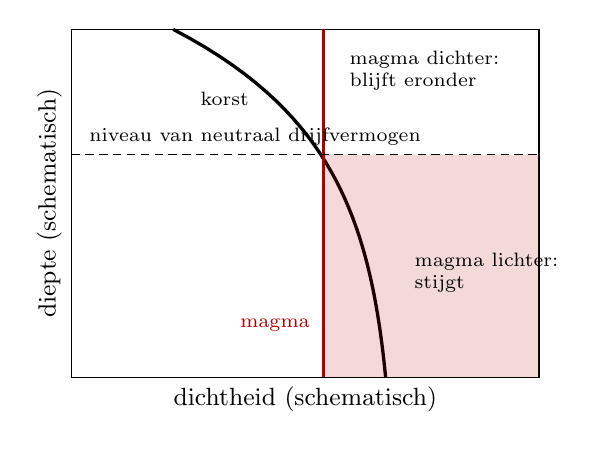
\begin{tikzpicture}[font=\scriptsize]
\begin{axis}[width=0.62\linewidth, height=6cm,
  xmin=0, xmax=1.15, ymin=0, ymax=1, y dir=reverse,
  xtick=\empty, ytick=\empty,
  xlabel={dichtheid (schematisch)}, ylabel={diepte (schematisch)},
  label style={font=\small}, clip=false]
\addplot[very thick, black, domain=0:1, samples=40] ({0.25 + 0.55*(1 - exp(-3*x))}, {x});
\addplot[very thick, red!70!black] coordinates {(0.62,0) (0.62,1)};
\fill[red!70!black, opacity=0.15] (axis cs:0.62,0.36) rectangle (axis cs:1.15,1);
\draw[densely dashed] (axis cs:0,0.36) -- (axis cs:1.15,0.36);
\node[anchor=south west] at (axis cs:0.02,0.36) {niveau van neutraal drijfvermogen};
\node[anchor=east, black] at (axis cs:0.46,0.20) {korst};
\node[anchor=east, red!70!black] at (axis cs:0.61,0.85) {magma};
\node[anchor=west, align=left] at (axis cs:0.82,0.70) {magma lichter:\\stijgt};
\node[anchor=west, align=left] at (axis cs:0.66,0.12) {magma dichter:\\blijft eronder};
\end{axis}
\end{tikzpicture}
\par\smallskip{\small Het \omterm{def:b2:magma-emplacement:ascent}{niveau van neutraal drijfvermogen} (schematisch). De dichtheid van
de korst neemt toe met de diepte, door compactie van sedimenten en door de overgang naar
dichtere gesteenten; een \omterm{def:b2:magma-emplacement:magma}{magma} met vaste dichtheid stijgt zolang het lichter is dan zijn
omgeving (gearceerd) en spreidt zich uit waar de twee dichtheden elkaar ontmoeten.}
\end{omfigure}

Een \omterm{def:b2:magma-emplacement:bodies}{pluton} moet ruimte voor zichzelf maken. Het kan zijn dak optillen, zoals een \omterm{def:b2:magma-emplacement:bodies}{laccoliet} doet;
het kan zijn wanden opzij duwen waar die zacht zijn; het kan ruimte vullen die door
breuken is geopend; en het kan zijn dak blok voor blok laten afbreken. Grote \omterm{def:b2:magma-emplacement:bodies}{plutonen} werden lang
voorgesteld als enorme magmatanks die in één keer werden geplaatst. Datering heeft dat
beeld veranderd. De zirkonen van de Tuolumne Intrusive Suite, een granietbatholiet in
Californië, tonen dat ze werd geplaatst tussen \num{95} en \qty{85}{Ma}, het oudst
aan de randen en het jongst in het centrum, en een van haar eenheden alleen al over meer
dan \qty{3}{Myr}, tussen \qty{92.8}{Ma} en \qty{88.8}{Ma}. Eén enkel magmalichaam
van \qty{5}{km} dik en \qty{20}{km} breed, geplaatst op \qty{15}{km} diepte, zou
onder \qty{750}{\celsius}, waar het ongeveer half gekristalliseerd is, zijn afgekoeld in
ongeveer \num{500000}~jaar. Zulke \omterm{def:b2:magma-emplacement:bodies}{plutonen} moeten stapsgewijs zijn opgebouwd,
uit veel kleinere intrusies zoals platen en \omterm{def:b2:magma-emplacement:bodies}{gangen}, over miljoenen jaren
(\cref{exo:b2:magma-emplacement:11}).
% ledger: glazner04:tuolumne

\begin{omfigure}
\centering
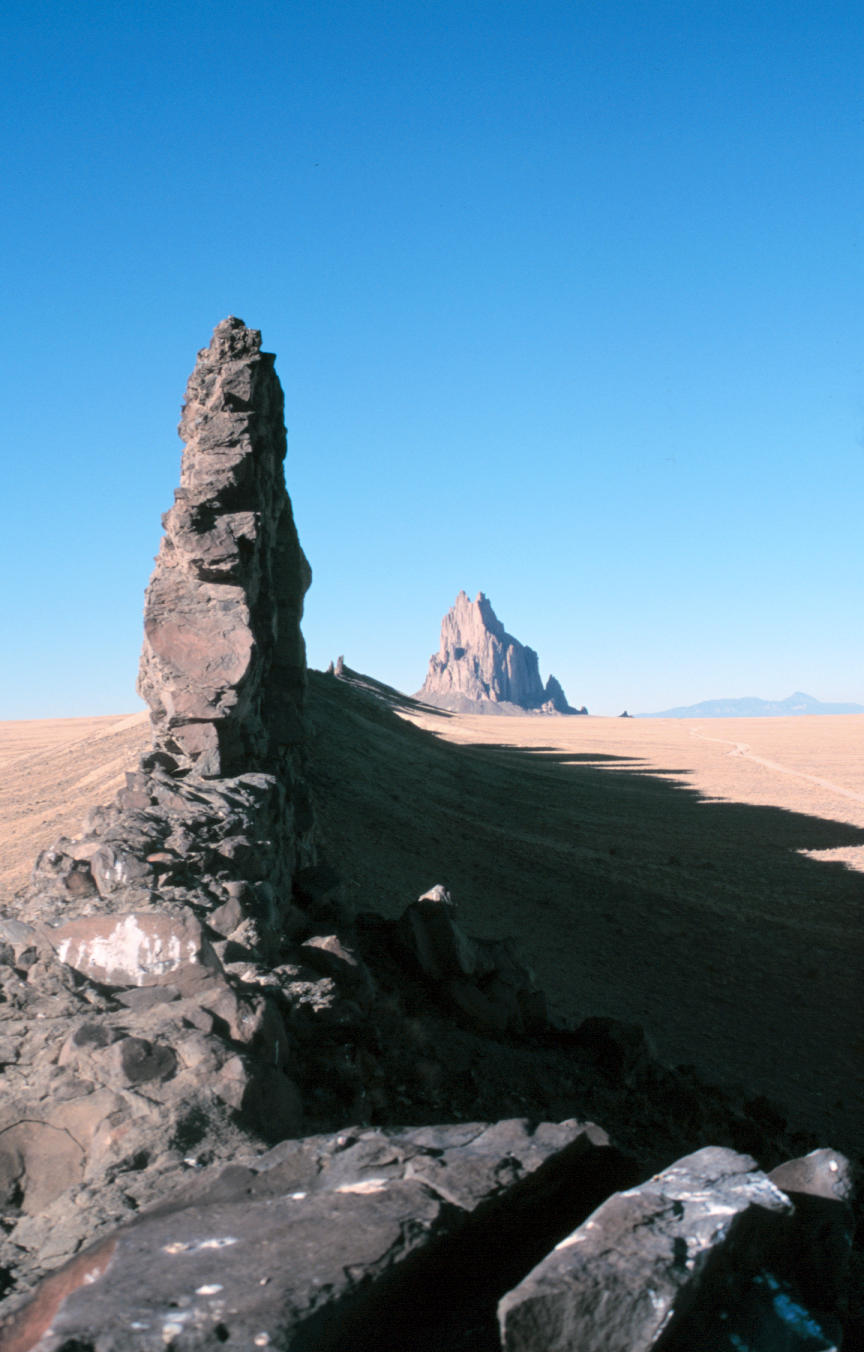
\includegraphics[width=0.3\linewidth]{images/book4/b2-shiprock-dyke.jpg}
\par\smallskip{\small Een \omterm{def:b2:magma-emplacement:bodies}{gang} bij Shiprock, in het Navajo Volcanic Field
(New Mexico): het ganggesteente weerstond de erosie beter dan de zandsteen en schalie
die het doorsneed, en staat nu als een muur; in de verte de vulkanische schoorsteen waaruit
meerdere zulke \omterm{def:b2:magma-emplacement:bodies}{gangen} uitstralen. Foto: Dexter Perkins (CC0).}
\end{omfigure}

\section{Afkoeling en contactmetamorfose}

Een intrusie verliest haar warmte door geleiding naar haar gastgesteenten. Het eenvoudigste
model behandelt de intrusie en haar gastgesteente als één geleidend medium met uniforme
diffusiviteit $\kappa$: op tijdstip nul heeft een plaat met dikte $b$ de
intrusietemperatuur $T_m$ en het gastgesteente $T_0$. De oplossing van de warmtevergelijking, met
$x$ gemeten vanaf het midden van de plaat, is
\[
T(x,t) = T_0 + \frac{T_m - T_0}{2}\left[\operatorname{erf}\frac{b/2 - x}{2\sqrt{\kappa t}}
+ \operatorname{erf}\frac{b/2 + x}{2\sqrt{\kappa t}}\right].
\]
De figuur hieronder toont ze voor een \omterm{def:b2:magma-emplacement:bodies}{sill} van \qty{100}{m} dik.
% ledger: delaney86b4:properties

\begin{proposition}[Contacttemperatuur]\label{prop:b2:magma-emplacement:contact}
In dit model blijft, zolang $\sqrt{\kappa t}$ klein is ten opzichte van $b$, de
temperatuur aan het contact van de intrusie op het gemiddelde $(T_m + T_0)/2$ van
de temperaturen van intrusie en gastgesteente.
\end{proposition}

\begin{proof}
Aan het contact $x = b/2$ is de eerste foutfunctie $\operatorname{erf}0 = 0$ en
de tweede $\operatorname{erf}(b/(2\sqrt{\kappa t}))$, die dicht bij $1$ ligt zolang
$b \gg 2\sqrt{\kappa t}$. Dan is $T = T_0 + (T_m - T_0)/2$.
\end{proof}

Een basaltgang van \qty{1150}{\celsius} in gesteenten van \qty{50}{\celsius} verhit zo
zijn contact tot \qty{600}{\celsius}. De kristallisatiewarmte, gewoonlijk
\qtyrange{700}{1000}{MJ/m^3}, houdt het \omterm{def:b2:magma-emplacement:magma}{magma} langer heet en verhoogt deze waarde:
met \qty{900}{MJ/m^3} die vrijkomt tussen \num{1150} en \qty{950}{\celsius}, geeft hetzelfde
model \qty{690}{\celsius}, terwijl temperatuurafhankelijke geleidbaarheden en natte
gastgesteenten beide schattingen met 50 tot \qty{75}{\celsius} verlagen.
% ledger: delaney86b4:dike, delaney86b4:properties

\begin{omfigure}
\centering
\begin{tikzpicture}
\begin{axis}[omrecord, width=0.86\linewidth, height=6cm,
  xmin=-200, xmax=200, ymin=0, ymax=1200,
  xlabel={afstand tot het midden van de sill (\unit{m})},
  ylabel={temperatuur (\unit{\celsius})},
  legend pos=north east, legend style={font=\scriptsize},
  tick label style={font=\scriptsize}, label style={font=\small}]
\fill[gray!15] (axis cs:-50,0) rectangle (axis cs:50,1200);
\addplot[very thick, red!80!black] table[x=x_m, y=t1] {figdata/out/bachelor-2-magma-sill.dat};
\addlegendentry{1 jaar}
\addplot[very thick, orange!90!black] table[x=x_m, y=t2] {figdata/out/bachelor-2-magma-sill.dat};
\addlegendentry{10 jaar}
\addplot[very thick, blue!60!black] table[x=x_m, y=t3] {figdata/out/bachelor-2-magma-sill.dat};
\addlegendentry{50 jaar}
\addplot[very thick, black] table[x=x_m, y=t4] {figdata/out/bachelor-2-magma-sill.dat};
\addlegendentry{200 jaar}
\draw[densely dashed, gray] (axis cs:-200,625) -- (axis cs:200,625);
\node[font=\scriptsize, gray!40!black, anchor=south west] at (axis cs:-198,625) {$(T_m + T_0)/2$};
\node[font=\scriptsize, anchor=south] at (axis cs:0,20) {sill};
\end{axis}
\end{tikzpicture}
\par\smallskip{\small Conductieve afkoeling van een \omterm{def:b2:magma-emplacement:bodies}{sill} van \qty{100}{m} dik (gearceerd),
geïntrudeerd bij \qty{1150}{\celsius} in gesteente van \qty{100}{\celsius}, met
$\kappa = \qty{0.7e-6}{m^2/s}$ en zonder latente warmte. Het contact blijft decennialang rond
\qty{625}{\celsius} terwijl de warmte zich in het gastgesteente verspreidt; na twee
eeuwen vormen de \omterm{def:b2:magma-emplacement:bodies}{sill} en zijn omgeving één brede warme zone.}
\end{omfigure}
% ledger: delaney86b4:properties

De tijdschaal van de afkoeling is de tijd die warmte nodig heeft om door de
intrusie te diffunderen, van de orde $(b/2)^2/\kappa$: ongeveer \num{16} dagen voor een \omterm{def:b2:magma-emplacement:bodies}{gang}
van \qty{2}{m} breed, een eeuw voor een \omterm{def:b2:magma-emplacement:bodies}{sill} van \qty{100}{m} dik, honderdduizend jaar
voor een \omterm{def:b2:magma-emplacement:bodies}{pluton} van enkele kilometers. De latente warmte verlengt ze, en ook de
noodzaak om het \omterm{def:b2:magma-emplacement:magma}{magma} te laten stollen in plaats van het alleen af te koelen.

\begin{proposition}[Stolling van een intrusie]\label{prop:b2:magma-emplacement:stefan}
Laat \omterm{def:b2:magma-emplacement:magma}{magma} op zijn stollingstemperatuur $T_m$, met latente warmte $L$ per volume-eenheid,
de ruimte $y > 0$ vullen naast een gastgesteente op $T_0$ dat $y < 0$ inneemt, beide
met warmtecapaciteit $\rho c$ per volume-eenheid en diffusiviteit $\kappa$. Het
stollingsfront schuift op als $y_s = 2\lambda\sqrt{\kappa t}$, waarbij $\lambda$
de wortel is van
\[
\frac{L\sqrt\pi}{\rho c\,(T_m - T_0)} = \frac{e^{-\lambda^2}}{\lambda\,(1 + \operatorname{erf}\lambda)},
\]
en het contact blijft op $T_0 + (T_m - T_0)/(1 + \operatorname{erf}\lambda)$. Een \omterm{def:b2:magma-emplacement:bodies}{sill}
met dikte $b$, die vanaf beide wanden stolt, is vast na
$t = b^2/(16\lambda^2\kappa)$.
\end{proposition}

\begin{proof}
Het \omterm{def:b2:magma-emplacement:magma}{magma} voor het front blijft op $T_m$, dus warmte stroomt alleen in de vaste stof
en het gastgesteente, waar de vorm $T = T_0 + (T_m - T_0)(1 + \operatorname{erf}\xi)/(1 +
\operatorname{erf}\lambda)$ met $\xi = y/(2\sqrt{\kappa t})$ wordt geprobeerd. Elke functie van $\xi$
van de vorm $\alpha + \beta\operatorname{erf}\xi$ lost de warmtevergelijking op; deze
nadert $T_0$ ver in het gastgesteente ($\xi \to -\infty$) en is gelijk aan $T_m$ op het front
$\xi = \lambda$. Bij $y = 0$ geeft ze de genoemde contacttemperatuur. Op het front
moet de latente warmte die de oprukkende vaste stof vrijmaakt, $L\,dy_s/dt = L\lambda\sqrt{\kappa/t}$
per oppervlakte- en tijdseenheid, worden afgevoerd, $k\,\partial T/\partial y = k(T_m -
T_0)\,e^{-\lambda^2}/[(1 + \operatorname{erf}\lambda)\sqrt{\pi\kappa t}]$. Gelijkstellen van de
twee en gebruik van $k = \rho c\kappa$ geeft de vergelijking voor $\lambda$. Elke wand van de
\omterm{def:b2:magma-emplacement:bodies}{sill} laat zijn eigen front groeien, onafhankelijk zolang de kern op $T_m$ blijft; de twee
fronten ontmoeten elkaar als $2\lambda\sqrt{\kappa t} = b/2$.
\end{proof}

Met de latente warmte van een basalt en een gastgesteente van ongeveer \qty{100}{\celsius}
is $\lambda$ ongeveer $0.65$: een \omterm{def:b2:magma-emplacement:bodies}{sill} van \qty{100}{m} dik stolt in ongeveer
zeventig jaar, en zijn contact blijft intussen rond \qty{740}{\celsius} in plaats van
\qty{625}{\celsius}. Het weekendprobleem werkt dit geval uit.
Omdat de tijd groeit met het kwadraat van de dikte, doet een tien keer dikkere \omterm{def:b2:magma-emplacement:bodies}{sill}
er honderd keer langer over.

\begin{definition}[Contacthof en zijn gesteenten]\label{def:b2:magma-emplacement:aureole}
Een \emph{afschrikrand}\index{afschrikrand} is de fijnkorrelige of glasachtige rand van een
intrusie, waar het \omterm{def:b2:magma-emplacement:magma}{magma} snel afkoelde tegen kouder gastgesteente. Een
\emph{contacthof}\index{contacthof} is de zone van gastgesteente rond een
intrusie die door haar warmte werd gemetamorfoseerd. \emph{Hoornrots}\index{hoornrots} is het
harde, fijnkorrelige, niet-gefolieerde gesteente waarin moddersteen en vulkanische gesteenten veranderen in
een contacthof. \emph{Skarn}\index{skarn} is het gesteente dat ontstaat waar hete magmatische
fluïda reageren met carbonaatgastgesteente en
calcium--ijzer--magnesiumsilicaten zoals granaat en pyroxeen afzetten, vaak met magnetiet en metaalsulfiden.
\end{definition}
% ledger: earle:intrusive-bodies, earle:skarn

Contacthoven variëren van enkele centimeters rond kleine \omterm{def:b2:magma-emplacement:bodies}{gangen} en \omterm{def:b2:magma-emplacement:bodies}{sills} tot
enkele tientallen meters rond een grote stock, en contactmetamorfose beslaat
ongeveer \qty{300}{\celsius} tot meer dan \qty{800}{\celsius}. Een moddersteen wordt een
\omterm{def:b2:magma-emplacement:aureole}{hoornrots}, een kalksteen een marmer, een zandsteen een kwartsiet. Een \omterm{def:b2:magma-emplacement:magma}{magma} dat diep
wordt geplaatst in gesteenten die al heet zijn, vormt bijna geen \omterm{def:b2:magma-emplacement:aureole}{contacthof}: de breedte hangt af van de
grootte en temperatuur van de intrusie en van de temperatuur van haar gastgesteente, zoals
het afkoelingsmodel voorspelt (\cref{exo:b2:magma-emplacement:12}). De mineralen die in een \omterm{def:b2:magma-emplacement:aureole}{contacthof} groeien,
en wat ze over de temperatuur zeggen, horen bij \cref{ch:b2:metamorphic-facies};
de metalen die \omterm{def:b2:magma-emplacement:aureole}{skarns} concentreren, bij \cref{ch:b2:ore-deposits}.
% ledger: earle:skarn

\begin{inthefield}[De contacten van een gang lezen]
\begin{minipage}[t]{0.6\linewidth}\vspace{0pt}
Waar een \omterm{def:b2:magma-emplacement:bodies}{gang} dagzoomt, volgt een geoloog eerst zijn contacten met het
gastgesteente. Een rand die fijnkorreliger of glasachtiger is dan het centrum van de \omterm{def:b2:magma-emplacement:bodies}{gang}, toont
dat het \omterm{def:b2:magma-emplacement:magma}{magma} tegen koud gesteente werd afgeschrikt; een \omterm{def:b2:magma-emplacement:bodies}{gang} van \qty{25}{cm} breed die
aan de kust van Brits-Columbia werd bestudeerd, heeft \omterm{def:b2:magma-emplacement:aureole}{afschrikranden} van \qty{2}{cm} dik. Het
gastgesteente naast het contact wordt onderzocht op verhitting: een kleurverandering, een verharding,
nieuwe mineralen die van de \omterm{def:b2:magma-emplacement:bodies}{gang} weg vervagen. De breedte van de verhitte zone en van
de \omterm{def:b2:magma-emplacement:aureole}{afschrikrand}, gemeten ten opzichte van de breedte van de \omterm{def:b2:magma-emplacement:bodies}{gang}, geeft aan hoe heet
het gastgesteente was toen de \omterm{def:b2:magma-emplacement:bodies}{gang} aankwam; een \omterm{def:b2:magma-emplacement:bodies}{gang} zonder \omterm{def:b2:magma-emplacement:aureole}{afschrikrand} en zonder
\omterm{def:b2:magma-emplacement:aureole}{contacthof} drong binnen in gesteenten die al heet waren. Er worden monsters genomen dwars over
de \omterm{def:b2:magma-emplacement:bodies}{gang}, van rand tot centrum, voor de geochemie van zijn smelt en voor de
grootte van zijn kristallen.
\end{minipage}\hfill
\begin{minipage}[t]{0.36\linewidth}\vspace{0pt}
\centering
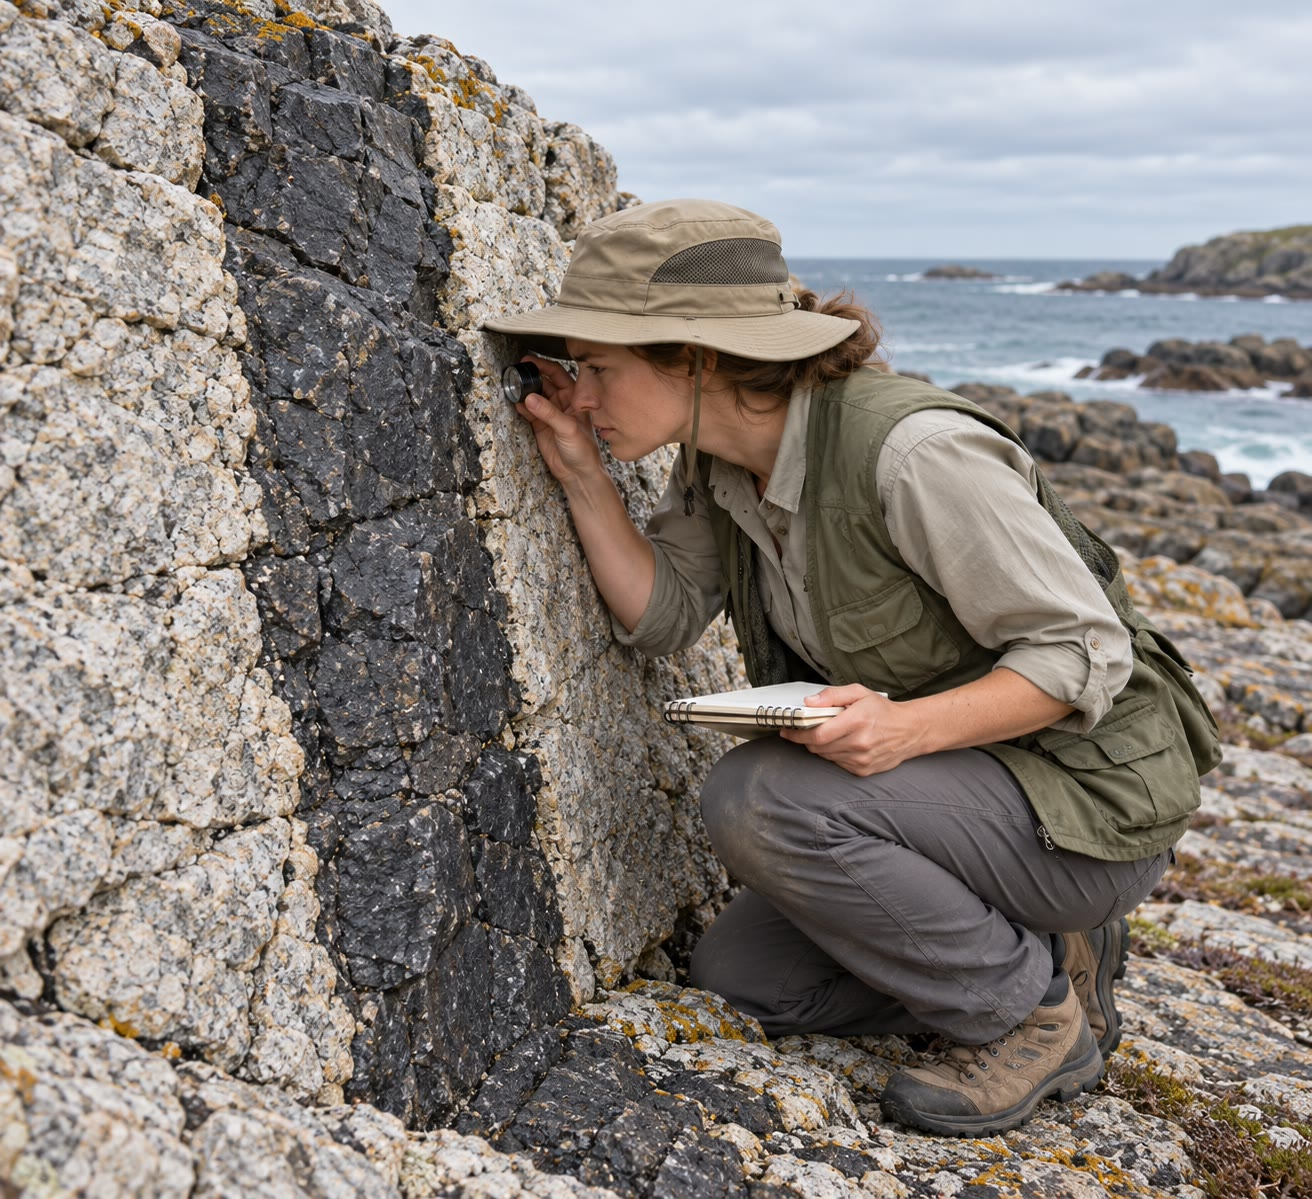
\includegraphics[width=\linewidth]{images/book4/ai/b2-dyke-contact.jpg}
\par\smallskip{\scriptsize Een geoloog onderzoekt het contact van een donkere \omterm{def:b2:magma-emplacement:bodies}{gang} met
licht gastgesteente (door AI gegenereerde illustratie).}
\end{minipage}
\end{inthefield}
% ledger: earle:intrusive-bodies

\section{Oefeningen}

\begin{exercise}[$\star$]\label{exo:b2:magma-emplacement:1}
Voor waterhoudende granitische smelten geeft een op metingen gefitte vergelijking
$\log_{10}\eta = [-3.545 + 0.833\ln w] + [9601 - 2368\ln w]/\{T - [195.7 + 32.25\ln
w]\}$, met $\eta$ in \unit{Pa.s}, $w$ het watergehalte in gewichtsprocent en $T$
in kelvin. Bereken $\log_{10}\eta$ bij \qty{800}{\celsius} voor $w = 1$ en $w = 4$,
en de factor waarmee de drie extra procent water de viscositeit verlagen.
\end{exercise}
% ledger: hd96:model

\begin{exercise}[$\star$]\label{exo:b2:magma-emplacement:2}
Bereken met de wortelwet, $s = 0.44$ voor een rhyoliet en $s = 0.34$ voor een basalt
(gewichtsprocent per $\sqrt{\unit{MPa}}$), de verzadigingsdruk van een
rhyoliet met \qty{6}{\percent} water en van een basalt met \qty{0.5}{\percent},
en de overeenkomstige diepten in een korst met dichtheid \qty{2600}{kg/m^3}
($g = \qty{9.81}{m/s^2}$).
\end{exercise}

\begin{exercise}[$\star$]\label{exo:b2:magma-emplacement:3}
Bereken de contacttemperatuur van een basaltgang van \qty{1150}{\celsius}
die in gesteenten van \qty{50}{\celsius} is geïntrudeerd, en daarna in gesteenten van
\qty{400}{\celsius}. Welke van de twee \omterm{def:b2:magma-emplacement:bodies}{gangen} krijgt de bredere \omterm{def:b2:magma-emplacement:aureole}{afschrikrand}?
\end{exercise}

\begin{exercise}[$\star$]\label{exo:b2:magma-emplacement:4}
Benoem elk lichaam. (a) Een plaat doleriet van \qty{30}{m} dik die tussen twee lagen
zandsteen ligt over \qty{20}{km}. (b) Een verticale plaat basalt van \qty{2}{m} breed
die horizontale kalkstenen doorsnijdt. (c) Een graniet die over \qty{2000}{km^2} dagzoomt,
opgebouwd uit een twaalftal eenheden van verschillende ouderdom. (d) Een lens porfier van \qty{1}{km} doorsnede,
vlak aan de basis, waarboven de lagen opgebold zijn. (e) Een horizontale plaat
basalt in een graniet.
\end{exercise}

\begin{exercise}[$\star\star$]\label{exo:b2:magma-emplacement:5}
Een basaltsmelt heeft $\eta_{\ell} = \qty{100}{Pa.s}$. Bereken met de relatie van
Einstein--Roscoe ($R = 1.35$) de viscositeit van het \omterm{def:b2:magma-emplacement:magma}{magma} met
\qty{5}{\percent}, \qty{20}{\percent}, \qty{40}{\percent} en \qty{60}{\percent}
kristallen, en vergelijk de eerste met de verdunde formule van Einstein. Bij welke
kristalfractie voorspelt de relatie vastlopen?
\end{exercise}

\begin{exercise}[$\star\star$]\label{exo:b2:magma-emplacement:6}
\omterm{def:b2:magma-emplacement:magma}{Magma} met een dichtheid die \qty{300}{kg/m^3} lager is dan die van zijn wanden, stijgt door een \omterm{def:b2:magma-emplacement:bodies}{gang} op.
(a) Bereken voor een basalt ($\eta = \qty{100}{Pa.s}$, $\rho = \qty{2700}{kg/m^3}$) in een \omterm{def:b2:magma-emplacement:bodies}{gang}
van \qty{1}{m} breed de gemiddelde snelheid, het debiet per meter \omterm{def:b2:magma-emplacement:bodies}{gang}, het
reynoldsgetal en de tijd om \qty{10}{km} te stijgen. (b) Dezelfde tijd voor een rhyoliet van
\qty{e6}{Pa.s} in een \omterm{def:b2:magma-emplacement:bodies}{gang} van \qty{1}{m} breed, daarna van \qty{10}{m} breed. (c) Een \omterm{def:b2:magma-emplacement:bodies}{gang}
van \qty{1}{m} breed verliest zijn warmte in een tijd van de orde $(w/2)^2/\kappa$, met $\kappa =
\qty{1e-6}{m^2/s}$: welke van de drie opstijgingen kan slagen?
\end{exercise}

\begin{exercise}[$\star\star$]\label{exo:b2:magma-emplacement:7}
Een \omterm{def:b2:magma-emplacement:magma}{magma} met dichtheid \qty{2400}{kg/m^3} bij \qty{900}{\celsius} geeft
\qty{1}{\percent} van zijn massa af als waterdamp. Bereken, met de damp als ideaal gas
($R = \qty{8.314}{J/(mol.K)}$, \qty{18.015}{g/mol}), de volumefractie
gas in het \omterm{def:b2:magma-emplacement:magma}{magma} bij \qty{100}{MPa}, \qty{10}{MPa} en \qty{0.1}{MPa}. Welke van de
drie waarden is het minst betrouwbaar, en waarom?
\end{exercise}

\begin{exercise}[$\star\star$]\label{exo:b2:magma-emplacement:8}
In een bekken neemt de dichtheid van de gesteenten toe met de diepte $z$ als $\rho(z) =
2300 + 60\,z$ (\unit{kg/m^3}, $z$ in \unit{km}) tot \qty{10}{km}. (a) Waar ligt
het \omterm{def:b2:magma-emplacement:ascent}{niveau van neutraal drijfvermogen} van een basaltsmelt van \qty{2650}{kg/m^3}? (b) Het
dichtheidsmodel van dit hoofdstuk toont dat één procent opgelost water
de dichtheid van een basaltsmelt met ongeveer \qty{70}{kg/m^3} verlaagt. Waar stopt een smelt met
één procent water meer? (c) Wat is de opwaartse kracht per kubieke meter
van de droge smelt \qty{2}{km} onder zijn \omterm{def:b2:magma-emplacement:ascent}{niveau van neutraal drijfvermogen}?
\end{exercise}

\begin{exercise}[$\star\star$]\label{exo:b2:magma-emplacement:9}
Veronderstel dat een granietdiapier met straal \qty{1}{km} en dichtheidstekort
\qty{300}{kg/m^3} opstijgt door onderkorst met viscositeit \qty{e19}{Pa.s}. Bereken
zijn stokessnelheid (starre bol) in millimeter per jaar en de tijd om
\qty{10}{km} te stijgen. Vergelijk met de tijdschaal $a^2/\kappa$ van zijn afkoeling, met $\kappa
= \qty{1e-6}{m^2/s}$. Wat volgt daaruit?
\end{exercise}

\begin{exercise}[$\star\star\star$]\label{exo:b2:magma-emplacement:10}
Water lost in een smelt op als moleculen, $x_m = K_1 f$, en als
hydroxylgroepen, $x_{\mathrm{OH}}^2 = K_2 x_m$ (de zuurstof van de smelt in grote overmaat), zodat
het totale opgeloste water $x = x_m + x_{\mathrm{OH}}/2$ is. (a) Druk $x$ uit als
functie van $f$ en toon aan dat het zich gedraagt als $\sqrt f$ bij lage $f$ en als $f$ bij
hoge $f$. (b) Bij welke fugaciteit zijn de twee vormen van water even overvloedig? (c)
Bereken met $K_1 = \qty{1e-4}{MPa^{-1}}$ en $K_2 = 0.2$ die fugaciteit, en het
aandeel water dat als hydroxyl is opgelost bij \qty{100}{MPa}.
\end{exercise}

\begin{exercise}[$\star\star\star$]\label{exo:b2:magma-emplacement:11}
Een granietpluton van \qty{1000}{km^3} wordt opgebouwd over \qty{4}{Myr}. (a) Bereken
zijn gemiddelde magma-aanvoer in \unit{km^3} per jaar en in \unit{m^3} per seconde. (b) Eén
enkele \omterm{def:b2:magma-emplacement:bodies}{gang} van \qty{1}{km} lang en \qty{2}{m} breed, met een gemiddelde snelheid van
\qty{0.8}{m/s}, voedt hem: hoe lang zou de \omterm{def:b2:magma-emplacement:bodies}{gang} erover doen om het hele
\omterm{def:b2:magma-emplacement:bodies}{pluton} aan te voeren? Welke fractie van de \qty{4}{Myr} is dat? (c) Als het \omterm{def:b2:magma-emplacement:bodies}{pluton} is opgebouwd uit
platen van \qty{20}{m} dik en \qty{10}{km} bij \qty{10}{km} breed, hoeveel platen
zijn er nodig, en hoeveel tijd ligt er gemiddeld tussen twee ervan? (d) Hoe lang doet een plaat er,
met $\lambda = 0.65$ en $\kappa = \qty{0.7e-6}{m^2/s}$, over om te
stollen? Is het \omterm{def:b2:magma-emplacement:bodies}{pluton} ooit één groot magmalichaam?
\end{exercise}

\begin{exercise}[$\star\star\star$]\label{exo:b2:magma-emplacement:12}
Ver van een dunne \omterm{def:b2:magma-emplacement:bodies}{gang} met breedte $b$ (op afstanden $x \gg b$) werkt zijn warmte als een
ogenblikkelijke vlakke bron: $T - T_0 = (T_m - T_0)\,b\,e^{-x^2/(4\kappa
t)}/\sqrt{4\pi\kappa t}$. (a) Toon aan dat de temperatuur op afstand $x$ het hoogst is op
$t^* = x^2/(2\kappa)$, en dat deze hoogste stijging $\Delta T_{\max} = (T_m -
T_0)\,b/(x\sqrt{2\pi e})$ is. (b) Op welke afstand warmt het gesteente voor een \omterm{def:b2:magma-emplacement:bodies}{gang} van \qty{2}{m} breed met $T_m - T_0 =
\qty{1100}{K}$ hoogstens \qty{100}{K} op, en
wanneer ($\kappa = \qty{0.7e-6}{m^2/s}$)? (c) Waarom zijn de contacthoven van dunne \omterm{def:b2:magma-emplacement:bodies}{gangen} zo
smal?
\end{exercise}

\section{Probleem: De sill onder het plateau}

\begin{problem}[{Weekendprobleem --- een basaltmagma volgen van zijn
toevoergang tot een sill, zijn water, en de tijd die de sill nodig heeft om te stollen}]
\label{pb:b2:magma-emplacement:1}
Onder een denkbeeldig plateau rusten sedimenten (schalie en zandsteen) met een gemiddelde dichtheid van
\qty{2450}{kg/m^3} op \qty{3.0}{km} diepte op een kristallijn basement met een
dichtheid van \qty{2800}{kg/m^3}. Een basaltmagma steeg op van \qty{15}{km} door een \omterm{def:b2:magma-emplacement:bodies}{gang}
van \qty{2.0}{m} breed en spreidde zich langs de basis van de sedimenten uit als een \omterm{def:b2:magma-emplacement:bodies}{doleriet-sill}
van \qty{100}{m} dik. Gegevens: intrusietemperatuur \qty{1150}{\celsius};
viscositeitswet van de smelt $\log_{10}\eta = -4.55 + 5510/(T - 611)$ ($T$ in kelvin);
dichtheid van de smelt met zijn water \qty{2710}{kg/m^3}; \qty{20}{\percent} kristallen in volume
(Einstein--Roscoe, $R = 1.35$); opgelost water \qty{0.40}{\percent}, oplosbaarheid
$s = 0.34$ procent per $\sqrt{\unit{MPa}}$; temperatuur van het gastgesteente bij de \omterm{def:b2:magma-emplacement:bodies}{sill}
\qty{100}{\celsius}; $\kappa = \qty{0.7e-6}{m^2/s}$, $\rho c = \qty{2.5}{MJ/(m^3.K)}$,
latente warmte \qty{900}{MJ/m^3}, waarbij het \omterm{def:b2:magma-emplacement:magma}{magma} wordt behandeld alsof het stolt op zijn
intrusietemperatuur; $g = \qty{9.81}{m/s^2}$; één jaar is \qty{3.156e7}{s}.

\medskip\noindent\textbf{Deel I --- Het magma.}
\begin{enumerate}
\item Bereken $\log_{10}\eta$ en $\eta$ van de smelt bij \qty{1150}{\celsius}
(\qty{1423}{K}).
\item Hetzelfde bij \qty{1100}{\celsius}. Met welke factor verandert de viscositeit over
deze \qty{50}{K}?
\item Bereken de viscositeit van het \omterm{def:b2:magma-emplacement:magma}{magma} met zijn kristallen bij
\qty{1150}{\celsius}.
\item Bij welke kristalfractie zou de relatie van Einstein--Roscoe het
\omterm{def:b2:magma-emplacement:magma}{magma} doen vastlopen? Vergelijk met de veldschatting van het einde van de stroming in bulk.
\item Bereken het dichtheidsverschil tussen het \omterm{def:b2:magma-emplacement:magma}{magma} en het basement, en
tussen het \omterm{def:b2:magma-emplacement:magma}{magma} en de sedimenten.
\item Bereken de lithostatische druk op het niveau van de \omterm{def:b2:magma-emplacement:bodies}{sill}.
\end{enumerate}

\noindent\textbf{Deel II --- Omhoog door de gang.}
\begin{enumerate}[resume]
\item Bereken de drukgradiënt van de opwaartse kracht, $\Delta\rho\,g$, die het \omterm{def:b2:magma-emplacement:magma}{magma}
door het basement drijft.
\item Bereken de gemiddelde snelheid van het \omterm{def:b2:magma-emplacement:magma}{magma} in de \omterm{def:b2:magma-emplacement:bodies}{gang}.
\item Bereken het debiet per meter \omterm{def:b2:magma-emplacement:bodies}{gang}, en het totale debiet als de \omterm{def:b2:magma-emplacement:bodies}{gang}
\qty{1.0}{km} lang is.
\item Bereken het reynoldsgetal van de stroming. Is ze laminair?
\item Hoe lang doet het \omterm{def:b2:magma-emplacement:magma}{magma} erover om van \qty{15}{km} tot \qty{3.0}{km} te stijgen?
\item Vergelijk met de tijdschaal $(w/2)^2/\kappa$ waarover de \omterm{def:b2:magma-emplacement:bodies}{gang} zijn
warmte verliest. Kan hij open blijven?
\item Leg uit waarom het \omterm{def:b2:magma-emplacement:magma}{magma} op \qty{3.0}{km} stopte en zich zijwaarts uitspreidde, met
de woordenschat van het hoofdstuk.
\end{enumerate}

\noindent\textbf{Deel III --- Het water.}
\begin{enumerate}[resume]
\item Bereken de verzadigingsdruk van het water van de smelt, en de diepte in de
sedimenten waar ze wordt bereikt.
\item Hoeveel water zou de smelt op het niveau van de \omterm{def:b2:magma-emplacement:bodies}{sill} kunnen bevatten? Ontmengt het
\omterm{def:b2:magma-emplacement:magma}{magma} van de \omterm{def:b2:magma-emplacement:bodies}{sill} water?
\item Blaasjes in de \omterm{def:b2:magma-emplacement:aureole}{afschrikrand} van de \omterm{def:b2:magma-emplacement:bodies}{sill} bevatten vooral CO$_2$. Verklaar.
\item Als alle \qty{0.40}{\percent} water aan het oppervlak vrijkwam, bij
\qty{1150}{\celsius} en \qty{0.1}{MPa}, welke volumefractie van het \omterm{def:b2:magma-emplacement:magma}{magma} zou
de damp dan innemen (ideaal gas)?
\end{enumerate}

\noindent\textbf{Deel IV --- Afkoeling en stolling.}
\begin{enumerate}[resume]
\item Bereken, zonder latente warmte, de contacttemperatuur van de \omterm{def:b2:magma-emplacement:bodies}{sill}.
\item Bereken, zonder latente warmte, de temperatuur \qty{10}{m} boven het bovenste
contact \num{10}~jaar na de intrusie.
\item Hetzelfde model: bereken de temperatuur in het midden van de \omterm{def:b2:magma-emplacement:bodies}{sill} na
\num{10}~jaar en \num{50}~jaar.
\item Hetzelfde model: bereken \qty{80}{m} boven het bovenste contact de temperatuur na
\num{300}, \num{363} en \num{420} jaar. Bereikt het gesteente daar ooit
\qty{300}{\celsius}?
\item Bereken $L\sqrt\pi/(\rho c\,(T_m - T_0))$ voor de \omterm{def:b2:magma-emplacement:bodies}{sill}.
\item Bereken $e^{-\lambda^2}/(\lambda(1 + \operatorname{erf}\lambda))$ voor $\lambda = 0.64$,
$0.65$ en $0.66$ ($\operatorname{erf}0.64 = 0.6346$, $\operatorname{erf}0.65 = 0.6420$,
$\operatorname{erf}0.66 = 0.6494$), en geef $\lambda$ tot op twee decimalen.
\item Bereken, met latente warmte, de contacttemperatuur terwijl de \omterm{def:b2:magma-emplacement:bodies}{sill}
stolt. Waarom is ze hoger dan in vraag 18?
\item Bereken de tijdschaal $(b/2)^2/\kappa$ in jaren.
\item Bereken de tijd die de \omterm{def:b2:magma-emplacement:bodies}{sill} nodig heeft om te stollen, in jaren, het kerngetal van
dit probleem, en leg uit waarom die korter is dan de tijdschaal van de vorige
vraag, hoewel er latente warmte moet worden afgevoerd.
\end{enumerate}
\end{problem}
% ledger: grd08:model, kolz22:einstein-roscoe, glazner04:tuolumne, moore98:h2o, lowenstern01:co2, delaney86b4:properties
